%%%%%%%%%%%%%%%%%%%%%%%%%%%%%%%%%%%%%%%%%%%%%%%%%%%%%%%%%%%%%%%%%%%%%%%%%%%%%%%%%%%%%%%%%%%%%%%%
%                                                                                              %
%                             Definicao para a classe Artigo                                   %
%                                                                                              %
%%%%%%%%%%%%%%%%%%%%%%%%%%%%%%%%%%%%%%%%%%%%%%%%%%%%%%%%%%%%%%%%%%%%%%%%%%%%%%%%%%%%%%%%%%%%%%%%

\documentclass[portugues, brazil, a4paper,12pt]{article}
\bibliographystyle{plain}

%%%%%%%%%%%%%%%%%%%%%%%%%%%%%%%%%%%%%%%%%%%%%%%%%%%%%%%%%%%%%%%%%%%%%%%%%%%%%%%%%%%%%%%%%%%%%%%%
%                                                                                              %
%                       Pacotes a utilizar na compilacao do documento                          %
%                                                                                              %
%%%%%%%%%%%%%%%%%%%%%%%%%%%%%%%%%%%%%%%%%%%%%%%%%%%%%%%%%%%%%%%%%%%%%%%%%%%%%%%%%%%%%%%%%%%%%%%%

\usepackage[brazil]{babel}
\usepackage{graphicx}
\usepackage{geometry}
\usepackage[utf8]{inputenc}
\usepackage[T1]{fontenc}
\usepackage{algorithm}
\usepackage{algorithmic}
\usepackage{verbatim} %blocos de comentario

%%%%%%%%%%%%%%%%%%%%%%%%%%%%%%%%%%%%%%%%%%%%%%%%%%%%%%%%%%%%%%%%%%%%%%%%%%%%%%%%%%%%%%%%%%%%%%%%
%                                                                                              %
%                       Configuracao dos pacotes utilizados no doc.                            %
%                                                                                              %
%%%%%%%%%%%%%%%%%%%%%%%%%%%%%%%%%%%%%%%%%%%%%%%%%%%%%%%%%%%%%%%%%%%%%%%%%%%%%%%%%%%%%%%%%%%%%%%%

\geometry{a4paper,left=3cm,right=3cm,top=2.5cm,bottom=2.93cm}


%%%%%%%%%%%%%%%%%%%%%%%%%%%%%%%%%%%%%%%%%%%%%%%%%%%%%%%%%%%%%%%%%%%%%%%%%%%%%%%%%%%%%%%%%%%%%%%%
%                                                                                              %
%                             Capa do relatorio tecnico                                        %
%                                                                                              %
%%%%%%%%%%%%%%%%%%%%%%%%%%%%%%%%%%%%%%%%%%%%%%%%%%%%%%%%%%%%%%%%%%%%%%%%%%%%%%%%%%%%%%%%%%%%%%%%

\begin{document}

\begin{titlepage}

  \vfill

\begin{figure}[H]
  \centering
  
\includegraphics[scale=0.45]{logo.jpg}
\end{figure}

  \vfill

  \begin{center}
    \begin{Large}
      \textbf{INSTITUTO FEDERAL DE EDUCAÇÃO, CIÊNCIA E TECNOLOGIA DE MINAS GERAIS}
    \end{Large}
  \end{center}

  \begin{center}
    \begin{large}
      \textbf{Bacharelado em Ciência da Computação e\\ Engenharia Elétrica} \\[1.4cm] 
    \end{large}
  \end{center}

  \vfill

  \begin{center}
    \begin{large}
      \textbf{Iniciação Científica: \\ Projeto e desenvolvimento de um carro robô controlado por smartphone, utilizando a plataforma Amarino \\ (Arduino e Google Android)} \\
      Relatório e Manual do Módulo Software no Google Android
    \end{large}
  \end{center}

  \vfill

  \begin{center}
    \begin{large}
      Alunos: \\
        João Paulo Fernandes de Cerqueira César - joaopaulofcc@gmail.com \\
		Rodolfo Labiapari Mansur Guimarães - rodolfolabiapari@gmail.com \\
		Tarlei Almeida - tarleialmeida@hotmail.com
    \end{large}
  \end{center}

\vfill

  \begin{center}
    \begin{large}
      Professores Orientadores: Prof. Otávio de Souza Martins Gomes e \\ Prof. Rafael Vinícius Tayette da Nobrega
    \end{large}
  \end{center}

\vfill

  \begin{center}
    \begin{large}
      Formiga - MG \\
      \today \\
    \end{large}
  \end{center}

\clearpage
\tableofcontents 
\end{titlepage}

%%%%%%%%%%%%%%%%%%%%%%%%%%%%%%%%%%%%%%%%%%%%%%%%%%%%%%%%%%%%%%%%%%%%%%%%%%%%%%%%%%%%%%%%%%%%%%%%
%                                                                                              %
%                               Nova Seção do Documento                                        %
%                                                                                              %
%%%%%%%%%%%%%%%%%%%%%%%%%%%%%%%%%%%%%%%%%%%%%%%%%%%%%%%%%%%%%%%%%%%%%%%%%%%%%%%%%%%%%%%%%%%%%%%%

%\newpage
%\section{Introdução}

\begin{comment}
\begin{figure}[H]
	\centering
	\includegraphics[scale=.1]{img/controle/controle/distancia.png}
	\caption{TEste}
	\label{fig:teste}
\end{figure}


\begin{figure}[H]
\centering
\begin{minipage}[c]{0.49\linewidth}
\centering
	\includegraphics[scale=.1]{img/controle/controle/distancia.png}
	\caption{TEste}
	\label{fig:teste}
\end{minipage}
\hfill
\begin{minipage}[c]{0.49\linewidth}
\centering
	\includegraphics[scale=.1]{img/controle/controle/distancia.png}
	\caption{TEste}
	\label{fig:teste}
\end{minipage}
\end{figure}


\begin{figure}[H]
	\centering
	\includegraphics[scale=.8]{img/controle/controle/.png}
	
\end{figure}


\begin{figure}[H]
\centering
\begin{minipage}[c]{0.49\linewidth}
\centering
	\includegraphics[scale=.8]{img/controle/controle/.png}
	
\end{minipage}
\hfill
\begin{minipage}[c]{0.49\linewidth}
\centering
	\includegraphics[scale=.8]{img/controle/.png}
	
\end{minipage}
\end{figure}

\end{comment}



%%%%%%%%%%%%%%%%%%%%%%%%%%%%%%%%%%%%%%%%%%%%%%%%%%%%%%%%%%%%%%%%%%%%%%%%%%%%%%%%%%%%%%%%%%%%%%%%
%                                                                                              %
%                               Nova Seção do Documento                                        %
%                                                                                              %
%%%%%%%%%%%%%%%%%%%%%%%%%%%%%%%%%%%%%%%%%%%%%%%%%%%%%%%%%%%%%%%%%%%%%%%%%%%%%%%%%%%%%%%%%%%%%%%%
\cite{tuto}
\newpage
\section{Módulo de Controle}

\subsection{Inicialização da Software}
O aplicativo possui procedimentos para inicialização de suas funções. Esses procedimentos são responsáveis pela primeira configuração, e tarefas que devem ser realizadas antes do funcionamento do aplicativo, para que esse opere corretamente.

\subsection{Variáveis}
Nas variáveis inicializadoras foram escolhidas as imagens de cada botão, valores de váriáveis, lógicas, textos exibidos no aplicativo, endereço do dispositivo pareado entre outros.

Ao abrir o aplicativo, o usuário se encontra na tela de controle do carro, para que ele possa então se conectar e usá-lo.

\begin{figure}[H]
	\centering
	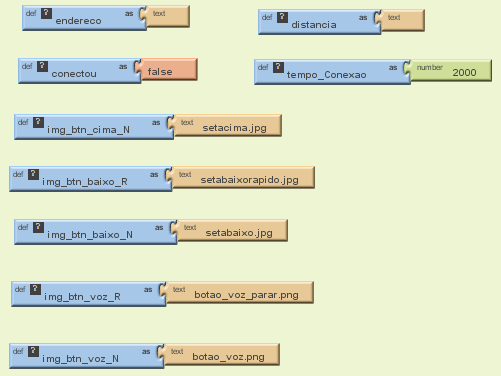
\includegraphics[scale=.8]{img/controle/variaveisPre.png}
	
\end{figure}

\subsection{Funções inicializadoras}
Foram utilizados eventos prévios específicos para controlar as ações do usuário. Por exemplo, a função \textit{Screen1.Initialize}, ela desativa a função \textit{sleep}\footnote{Função que faz uma pausa de alguns segundos por segurança na conexão.} pois só será necessário quando for solicitada a troca de telas, retira o campo que exibirá a distância pois este só deverá aparecer somente quando o usuário achar necessário.


\begin{figure}[H]
	\centering
	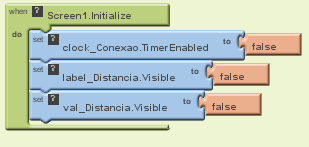
\includegraphics[scale=.8]{img/controle/screenInitialize.png}
	
\end{figure}

Ainda na inicialização se o usuário ainda não estiver com o \textit{Bluetooth} do dispositivo \textit{Android} habilitado será então mostrado a ele uma tela pedindo autorização para ativar o \textit{Bluetooth}. Caso o usuário não ative o \textit{Bluetooth}, o aplicativo não executará nenhuma função de controle, evitando assim um funcionamento incorreto no aplicativo.



\begin{figure}[H]
	\centering
	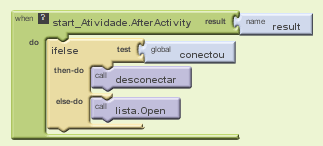
\includegraphics[scale=.8]{img/controle/screenInitialize1.png}
	
\end{figure}








%%%%%%%%%%%%%%%%%%%%%%%%%%%%%%%%%%%%%%%%%%%%%%%%%%%%%%%%%%%%%%%%%%%%%%%%%%%%%%%%%%%%%%%%%%%%%%%%
%                                                                                              %
%                               Nova Seção do Documento                                        %
%                                                                                              %
%%%%%%%%%%%%%%%%%%%%%%%%%%%%%%%%%%%%%%%%%%%%%%%%%%%%%%%%%%%%%%%%%%%%%%%%%%%%%%%%%%%%%%%%%%%%%%%%
\subsection{Principais Funções}

\subsubsection{Pareando}
O procedimento \textit{lista.BeforePicking} possui a função de exibir a lista de dispositivos preveamente pareados com o \textit{Android}.

Já o procedimento \textit{lista.AfterPicking}, recolhe o endereço do dispositivo escolhido pelo usuário e o armazena na variável responsável. Em seguida realiza a conexão dos dispositivos, informando o aplicativo que houve conexão, ativando assim o modo de operação do carro e o sensor ultrassônico.

\begin{figure}[H]
\centering
\begin{minipage}[c]{0.49\linewidth}
\centering
	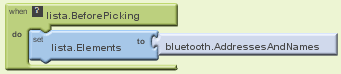
\includegraphics[scale=.8]{img/controle/antesConectar.png}
	
\end{minipage}
\hfill
\begin{minipage}[c]{0.49\linewidth}
\centering
	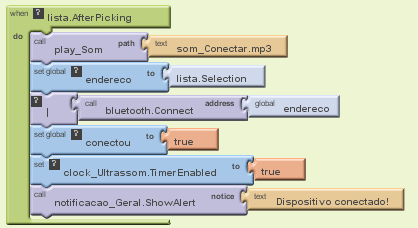
\includegraphics[scale=.8]{img/controle/depoisConectar.png}
	
\end{minipage}
\end{figure}


\subsubsection{Movimentação}
O movimento do carro para girar a direita, análogo aos outros (esquerda, frente, frente rápido, ré, ré rápido e pelos comandos de voz) é gerenciado por uma estrutura condicional que, após o acionamento do botão, verifica se o dispositivo está conectado com o carro. Caso contrário ele solicitará a conexão imediata. Conectado, ele fará com que o dispositivo, se for possível, vibre alertando a ação que será executada. Caso uma colisão com qualquer objeto que esteja em sua frente seja iminente, o aplicativo desconsidera qualquer ação previamente executada, e para o carro. Caso o usuário possua sintetizador de voz em seu dispositivo \textit{Android}, ele então ouvirá uma mensagem de alerta de colisão. Mas, se nenhum objeto o impedir, ele encarregará de enviar o comando para o carro robô a fim de promover a ação solicitada pelo usuário.

\begin{figure}[H]
	\centering
	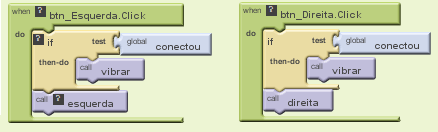
\includegraphics[scale=.8]{img/controle/fdireitaesquerda.png}
	
\end{figure}


\begin{figure}[H]
	\centering
	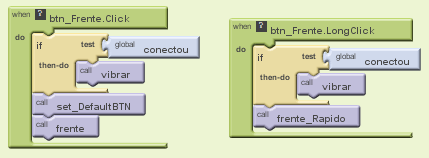
\includegraphics[scale=.8]{img/controle/ffrentes.png}
	
\end{figure}


\begin{figure}[H]
	\centering
	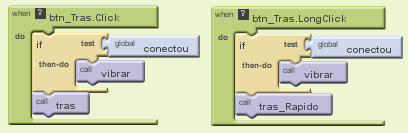
\includegraphics[scale=.8]{img/controle/ftras.png}
	
\end{figure}

\begin{figure}[H]
	\centering
	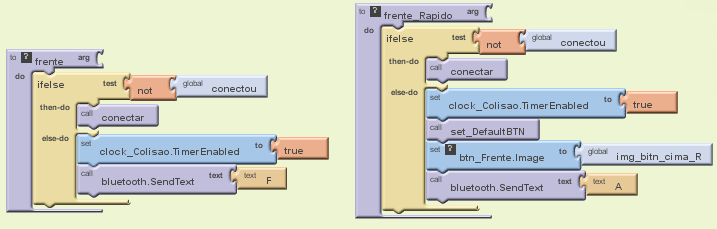
\includegraphics[scale=.8]{img/controle/frentes.png}
	
\end{figure}


\begin{figure}[H]
	\centering
	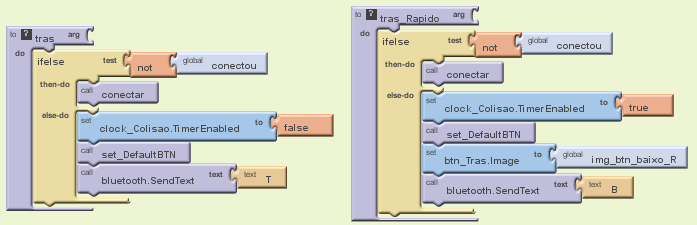
\includegraphics[scale=.8]{img/controle/tras.png}
	
\end{figure}



\begin{figure}[H]
	\centering
	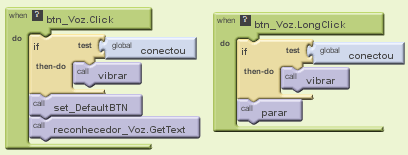
\includegraphics[scale=.8]{img/controle/fvoz.png}
	
\end{figure}

Deve-se lembrar que o clique \textbf{curto} no botão de comando de voz significa o \textit{\textbf{acionamento}} deste. Já o \textbf{clique longo}, \textit{\textbf{interrompe}} todos os movimentos feitos pelo carro. É utilizado como uma execução de \textit{emergência} do sistema.


\begin{figure}[H]
	\centering
	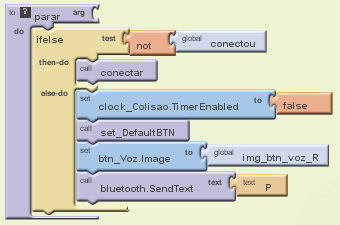
\includegraphics[scale=.8]{img/controle/parar.png}
	
\end{figure}



\subsubsection{Função de Reconhecimento de comandos vocais}
Uma função de reconhecimento de voz, específica, se encarregará de gravar, ao toque de um botão, o que o usuário falar de acordo com os requisistos de funcionamento, e promover a ação do carro somente com a voz do usuário.

Os requisistos de um bom funcionamento dependem diretamente de:

\begin{itemize}
	\item uma conexão com a Internet ou pacote de reconhecimento vocal \textit{off-line} da Google instalado;
	\item que não haja barulhos que possam atrapalhar o aplicativo gravar o comando;
	\item falar alto (não exagerando), um pouco devagar perante a velocidade de conversas informais e com o português correto e claro para o entendimento.
\end{itemize}



\subsubsection{Distância captada pelo sensor}
Procedimento responsável por enviar os dados do sensor ultrassônico através do \textit{Bluetooth} para o dispositivo \textit{Android} controlador do carro\cite{bt}.

\begin{figure}[H]
	\centering
	\includegraphics[scale=.7]{img/controle/distancia.png}
	
\end{figure}
A transmissão dos dados lidos por qualquer sensor que esteja conectado ao carro, é tranferida é realizada de modo que caracteres sejam enviados para entre os dispositivos formando um texto compreensível para o usuário no receptor. Porém o envio é realizado dividindo esse texto, enviando caracter por caracter ao dispositivo \textit{Android}. Portanto é necessário criar uma função que receba esses caracteres e monte novamente o texto original.

Com esta questão, no recebimento de pacotes da distância, há um monitoramento de quantidade de \textit{bytes} que são enviados do Arduino até o \textit{Android} como um todo. Enquanto houverem dados (caracteres) a serem recebidos pelo \textit{Bluetooth}, o aplicativo então lê esses dados, concatenando-os com as outras partes do dado anteriormente recebidas.

\begin{figure}[H]
	\centering
	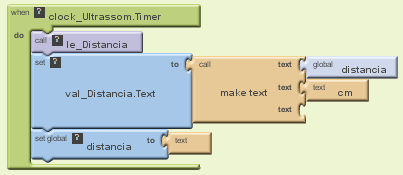
\includegraphics[scale=.8]{img/controle/ultrassom.png}
	
\end{figure}



\subsubsection{Vibração}
A vibração\footnote{Motor Elétrico que geralmente possui 15 x 5 milímetros e um eixo de metal em formato de meia-lua numa das pontas. Com a rotação, ele produz ocilações do dispositivo movél como um todo\cite{vibracall}.} é constantemente utilizada para concentrar o usuário em suas ações. Seu objetivo é que todo o cuidado ocorra em cada movimento solicitado. Foi definido como padrão o tempo de vibração de cem microssegundos ($ms$).


\begin{figure}[H]
	\centering
	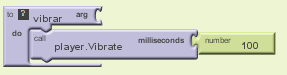
\includegraphics[scale=.8]{img/controle/vibrar.png}
	
\end{figure}


\subsubsection{Comando de voz `Quem é você?'}
Utilizando o comando de voz, é possível obter informações sobre o aplicativo e sobre os desenvolvedores do \textit{software}. Mencionando a frase \verb%Quem é você?% será possível escutar a seguinte mensagem caso o dispositivo \textit{Android} possua sintetizador de voz instalado:

\begin{verbatim}
Eu sou ADA, seu computador de bórdo!
Fui criada pelo C 2 I S C do I F M G campus Formiga
\end{verbatim}

\begin{figure}[H]
	\centering
	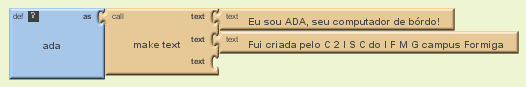
\includegraphics[scale=.9]{img/controle/textos.png}
	
\end{figure}


\subsubsection{Chama Monitoramento} 
Ao acionar qualquer botão que tem como sua finalidade a mundaça de tela, este é o primeiro procedimento a ser executado. Ele exibe uma notificação para o usuário aguardar, pois, é necessário aproximadamente dois segundos para a transição segura entre as páginas, devido a reconexão com o \textit{Bluetooth}.

\begin{figure}[H]
\centering
\begin{minipage}[c]{0.49\linewidth}
\centering
	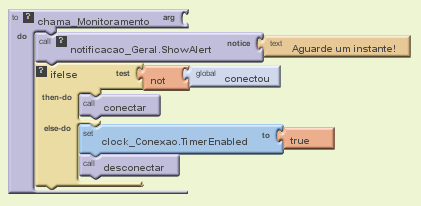
\includegraphics[scale=.8]{img/controle/monitoramento.png}
	
\end{minipage}
\hfill
\begin{minipage}[c]{0.49\linewidth}
\centering
	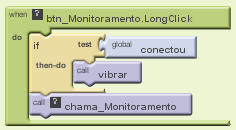
\includegraphics[scale=.8]{img/controle/monitoramentoLong.png}
	
\end{minipage}
\end{figure}

\subsubsection{Clock Conexão}
Este faz parte do procedimento monitoramento mencionado acima. Ele é uma extensão/complemento, pois, ao trocar para a tela de monitoramento é necessário que ele desconecte do dispositivo pareado. O \textit{MIT App Inventor} não permite acessar os componentes de outro tela, sendo assim preciso adicionar todos eles novamente na nova tela, isso faz com que seja necessária uma reconexão com o dispositivo pareado. Portanto esse procedimento é responsável por desconectar de forma segura do dispositivo pareado, e então abrir a nova tela para que nessa seja reconectado.

Para a assegurar a desconexão, achou-se necessário a espera de dois segundos. A cada cem milíssegundos ele executa todo a estrutura até verificar a contagem de dois segundos garantido a desconexão.

Quando sua contagem for igual a dois segundos ele então abre a nova tela. Ao fazer isso ele passa para tela chamada alguns valores, como, endereço do dispositivo para reconexão, e todos os textos usados em ambas as telas. Ao se passar como parâmetro o valor das variáveis que armazenam os textos, fica fácil uma manutenção futura, pois basta atualizar os seus valores na tela principal que esses também serão atualizados na tela na programação da tela de controle de monitoramento.

\begin{figure}[H]
	\centering
	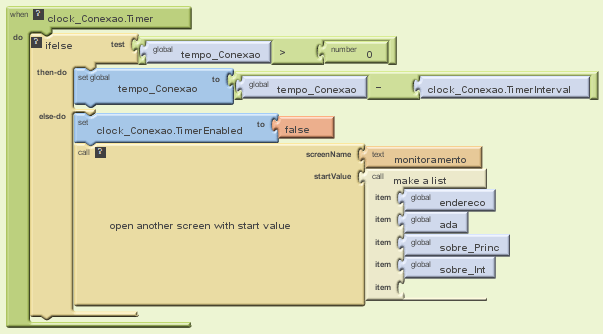
\includegraphics[scale=.8]{img/controle/clockconexao.png}
	
\end{figure}


\subsubsection{Imagens Padrão}
Este procedimento é único e exclusivamente responsável por retornar as imagens ao padrão. Ao clicar num botão, no movimento \textit{hover} dele (tocar no botão sem remover o dedo; `continar pressionando'), o usuário poderá notar que há uma diferença na coloração do botão, indicando perfeitamente qual o botão foi pressionado.

Quando, por exemplo, o usuário somente tocar em qualquer botão direcional ou de comando de voz, sua imagem não muda, isto é, o botão permanecerá com sua cor padrão, e o comando equivalente será executado. Porém existem botões com dupla função e que ao serem usados modificam a imagem desses, como, as setas direcionais frente e trás, o botão de reconhecimento de voz. Ao executarem essas ações, a cor do botão que foi pressionado, passará a ser vermelha, e então o comando específico será executado. Caso o usuário pressione outra tecla, sua cor voltará à padrão. É importante ressaltar, que os comandos são sempre do tipo permanente (ao executar a função de um botão, essa continuará até que ser interrompida por outro botão, o usuário pode tocar apenas uma vez no botão e retirar o dedo) e só executará outra função caso o usuário pressione outra tecla.


\begin{figure}[H]
	\centering
	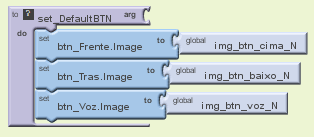
\includegraphics[scale=.8]{img/controle/defaultimg.png}
	
\end{figure}


\subsubsection{Exibe e esconde a Distância}
Ao comando do usuário, é possível que apareça na tela do dispositivo \textit{Android} uma etiqueta que exibirá o valor da distância em centímetros ($cm$), de qualquer objeto que esteja num intervalo de confiança captado pelo sensor entre 0 à 450 $cm$ (4,5 metros) da frente do carro.

Antes da função de distância ser ativada completamente, deve-se verificar se o dispositivo está conectado ao carro. Se sim, os comando serão ativados e aparecerá no aplicativo a etiqueta de \textit{distância} e a de \textit{valor} em centímetros.


\begin{figure}[H]
	\centering
	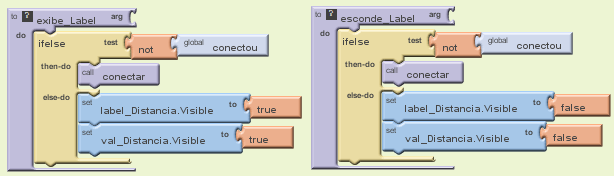
\includegraphics[scale=.8]{img/controle/exibeesconde.png}
	
\end{figure}

O mesmo vale para a desativação dos controles. Há a verificação de conexão para depois a desabilitação da etiqueta junto com seu valor, retirando estes do visor.



\subsubsection{Função Play Sound}
Sempre que o usuário fizer alguma função que for de importância ou de atenção será executado um som curto alertando de sua ação. Em cada evento terá um som diferente. Por exemplo, na conexão, nos direcionais, na desconexão e na página Sobre, terão sons breves e diferentes entre si, para que o usuário possa focar sua atenção no controle do carro.

\begin{figure}[H]
	\centering
	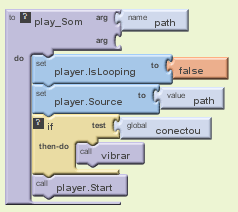
\includegraphics[scale=.8]{img/controle/som.png}
	
\end{figure}


O som é tocado apenas uma vez em cada ação do evento. Como em todas as outras funções, é verificado se o dispositivo está conectado para o envio da função para o carro. Caso sim, ele vibrará tocando a som predefina pelo programa no evento.


\subsubsection{Página Sobre}
Quando o usuário clicar sobre o ícone \verb%Sobre%, será redirecionado para a página específica, ainda pertencente ao aplicativo, que irá informar ao usuário detalhes gerais sobre o aplicativo, onde foi desenvolvido, autores de produção e de orientação mostrando todos os responsáveis.

\begin{figure}[H]
	\centering
	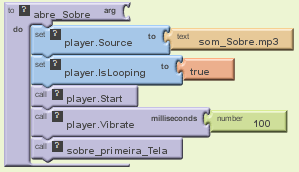
\includegraphics[scale=.8]{img/controle/sobremusica.png}
	
\end{figure}

%Somente na página \verb%Sobre%, foi adicionado uma canção da banda Pink Floyd alterada para o estilo de \textit{8-bit} repetindo sem pausa. Este, proposto pelos desenvolvedores que todo o projeto, foi feito por fins acadêmicos e de livre usabilidade para qualquer um, seguindo regras impostas pelos orientadores, de modo que a criatividade de seus projetistas não sejam limitadas mas sim direcionadas abrindo inúmeras possibilidades de variaçãos e melhorias de aplicativos trabalhando-se harmonicamente com o projeto e com a equipe independentemente do propósito final do projetista, do orientador ou da instituição local.


\begin{figure}[H]
	\centering
	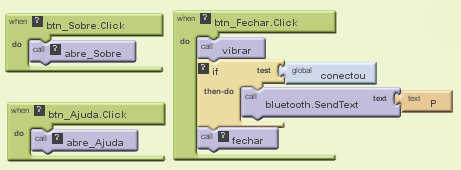
\includegraphics[scale=.8]{img/controle/paginas.png}
	
\end{figure}


\begin{verbatim}
Carduino é um aplicativo livre, criado pelo grupo de pesquisa 
C2ISC (Concepção de Circuitos Integrados e Sistemas de Comunicação) 
do IFMG campus Formiga.

O app é produto do projeto de pesquisa:
"Projeto e desenvolvimento de um carro robô controlado por Smartphone,
utilizando a plataforma Amarino (Arduino e Google Android)"
\end{verbatim}

\begin{figure}[H]
	\centering
	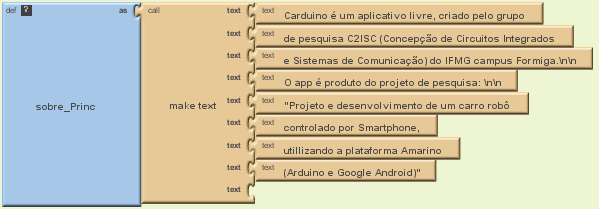
\includegraphics[scale=.8]{img/controle/textos1.png}
	
\end{figure}

E numa segunda tela:
\begin{verbatim}
Integrantes

Alunos:
João Paulo FCC - 4 P - C.C.
Rodolfo Labiapari - 4 P - C.C.
Tarlei Almeida - 4 P - E.E.

Orientador:

Otávio de Souza Martins Gomes
Coorientador:

Rafael Tayette da Nobrega

Novembro de 2013
Formiga/MG
\end{verbatim}

\begin{figure}[H]
	\centering
	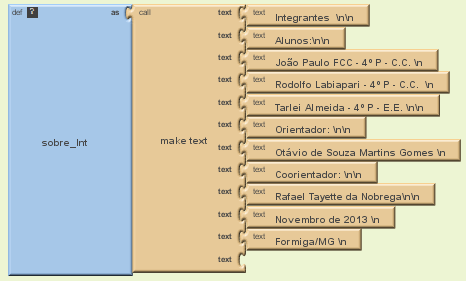
\includegraphics[scale=.8]{img/controle/textos2.png}
	
\end{figure}

\begin{figure}[H]
	\centering
	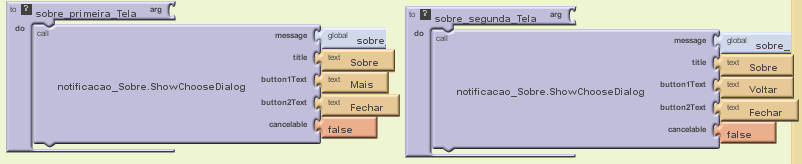
\includegraphics[scale=.8]{img/controle/sobre1.png}
	
\end{figure}


\begin{figure}[H]
	\centering
	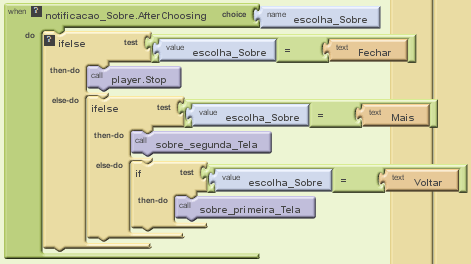
\includegraphics[scale=.8]{img/controle/sobre2.png}
	
\end{figure}

Existem três botões nesta janela que será aberta, os botões \verb%Sobre%, \verb%Mais% e \verb%Fechar%. Como o texto relatando o produto final do software é extenso, foi necessário dividi-lo em duas telas que serão acorrentadas através do botão chamado \verb%Mais% e o de retorno \verb%Voltar%.


\subsubsection{Página Ajuda}
Igualmente ao evento de redirecionamento da página \verb%Sobre%, o usuário será redirecionado a página de \verb%Ajuda% do aplicativo. %Será exibido o seguinte texto para auxiliar o usuário no controle do carro:

\begin{figure}[H]
	\centering
	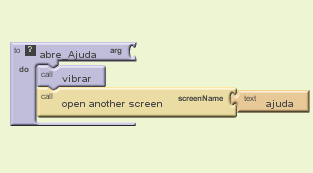
\includegraphics[scale=.8]{img/controle/ajuda.png}
	
\end{figure}


\subsubsection{Procedimento Anti-Colisão}
A colisão com objetos é algo que não poderá acontecer ao carro. Então, para tentar diminuir o seu risco adicionou-se em seu projeto um sensor ultrassônico na dianteira (frente) do carro para que, de tempos em tempos, monitore constantemente a distância de obstáculos. A sua capacidade de reconhecer um objeto em um intervalo de confiança é de 4 à 4,5 metros\footnote{Descritos nas especificações de \textit{hardware} do dispositivo ultrassônico.}. Então decidiu-se que qualquer obstáculo que estiver em uma distância igual ou menor que quize centímentros da dianteira do carro acionará automáticamente um comando que abortará qualquer movimento que o carro estiver fazendo.

Caso o sensor detecte algum objeto na distância predefinida, ele exibirá uma etiqueta e se caso o dispositivo tenha o sintetizador de voz instalado o executará um som que dirá \verb%Atenção!% ao parar o carro evitando danos, caso ele tenha o sintetizador de voz.

\begin{figure}[H]
	\centering
	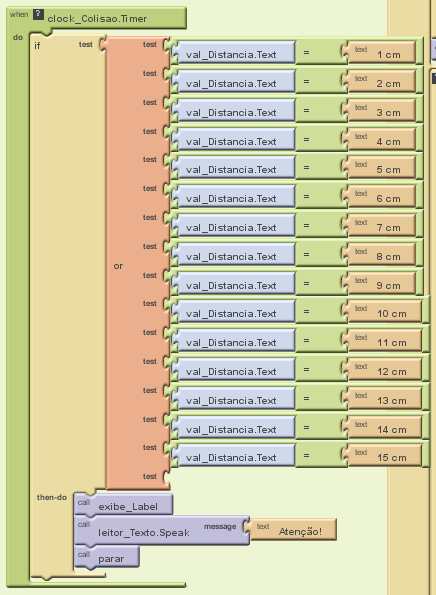
\includegraphics[scale=.8]{img/controle/colisao.png}
	
\end{figure}


\subsubsection{Fala Distância}
O usuário também tem como uma escolha a opção que o aplicativo `fale/pronuncie' a distância para ele. Devido esta interatividade o aplicativo se torna dinâmico e de fácil execução pelo usuário, incrementanto a interatividade a percepção e necessidade do usuário. É necessário lembrar que para o funcionamento deste recurso, o dispositivo deve possuir o sintetizador de voz instalado no dispositivo.

Após verificado se o dispositivo está perfeitamente conectado, o sintetizador reproduz o valor para o usuário.

\begin{figure}[H]
	\centering
	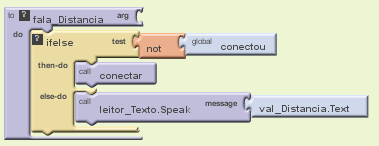
\includegraphics[scale=.8]{img/controle/distanciaFala.png}
	
\end{figure}

\subsubsection{Desempareamento}
Um dos procedimentos pricipais é a desconexão entre os dispositivos.

A desconexão segura entre os dispositivos é altamente importante para que ambos possam se conectar com outros dispositivos (o dispositivo \textit{Android} em um fone de ouvido e o carro em outro dispositivo \textit{Android} qualquer por exemplo).

Ao executar o evento, se o dispositivo já estiver desconectado, o aplicativo notifica o usuário informando que o dispositivo não está conectado. Caso contrário, o dispositivo notifica o usuário alertando-o que a desconexão foi realizada com sucesso. Inicia-se então o processo de interromper qualquer movimento que o carro estiver realizando, e deixa de realizar leituras do sensor ultrassônico. Isso fornece ao aplicativo um nível a mais de segurança, na medida que o carro ficará estacionado aguardando uma nova conexão ao invés de continuar movimentos sem controle.

\begin{figure}[H]
	\centering
	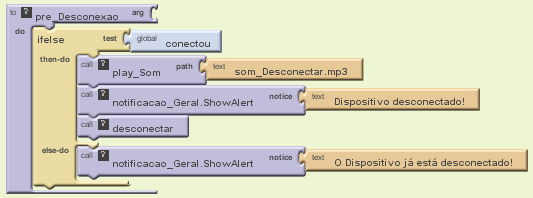
\includegraphics[scale=.8]{img/controle/desconexao.png}
	
\end{figure}

\begin{figure}[H]
	\centering
	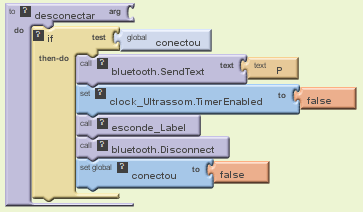
\includegraphics[scale=.8]{img/controle/desconectar.png}
	
\end{figure}


\subsubsection{Fechando telas}
Este procedimento é executado quando qualquer janela chamada a partir da tela de controle é fechada. Quando isso ocorre, algumas medidas devem ser tomadas.

Ao fechar a janela chamada anteriormente retorna como parâmetro para a tela principal o endereço do dispositivo \textit{Bluetooth} que estava conectado. A variável controladora da função \textit{sleep} é reconfigurada para seu valor original, pois quando a tela principal chama uma outra tela este valor é zerado.

É necessário também que ocorra uma reconexão entres os dispositivos, utilizando o valor passado por parâmetro. Feito isso, é sinalizada a conexão e ativado a leitura dos dados do sensor.

Tudo que for chamado pela página de controle, terá que seguir este procedimento pois ele controla o \textit{Bluetooth} para que continue funcionando perfeitamente. Após dois segundos ele confirma a conexão e retorna ativo o ultrassom.


\begin{figure}[H]
	\centering
	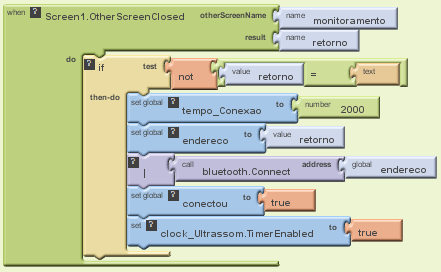
\includegraphics[scale=.8]{img/controle/fotherscreen.png}
	
\end{figure}


\subsubsection{Encerramento do Programa}

No encerramento do aplicativo, foi utilizado uma sequência de perguntas para confirmar a opção do usuário. 

Essa prática foi utilizada pela razão dos controles serem apenas em telas \textit{touch screen} abrangendo a probabilidade em que o usuário toque no botão sem a real intenção, possibilitando que ele retorne ao mesmo ponto em que ele estava sem qualquer prejuízo.

\begin{description}
\item[Mensagem: ]Você deseja realmente sair do aplicativo?
\item[Botões: \quad\,\,\,\,](Sim) (Não)
\end{description}

Qualquer cancelamento nesta área será redirecionado a tela do aplicativo onde havia parado (área de controle do carro). Mas quando o usuário responder que deseja sair, o aplicativo irá parar qualquer movimento do carro robô, se desconectará do carro automaticamente e em seguida fechará o aplicativo voltando para o Sistema Operacional do dispositivo (área de trabalho do aparelho).


\begin{figure}[H]
	\centering
	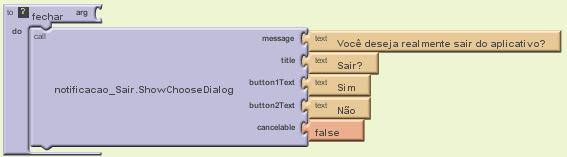
\includegraphics[scale=.8]{img/controle/fechar.png}
	
\end{figure}



%%%%%%%%%%%%%%%%%%%%%%%%%%%%%%%%%%%%%%%%%%%%%%%%%%%%%%%%%%%%%%%%%%%%%%%%%%%%%%%%%%%%%%%%%%%%%%%%
%                                                                                              %
%                               Nova Seção do Documento                                        %
%                                                                                              %
%%%%%%%%%%%%%%%%%%%%%%%%%%%%%%%%%%%%%%%%%%%%%%%%%%%%%%%%%%%%%%%%%%%%%%%%%%%%%%%%%%%%%%%%%%%%%%%%

\newpage
\section{Página Ajuda}
\subsection{Exibe textos de Suporte ao usuário}
Ao iniciar a página será executado o procedimento responsável por inicializar e comandar os outros eventos.

\begin{figure}[H]
	\centering
	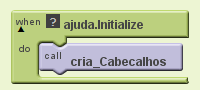
\includegraphics[scale=.8]{img/ajuda/inicio.png}
	
\end{figure}

\begin{figure}[H]
	\centering
	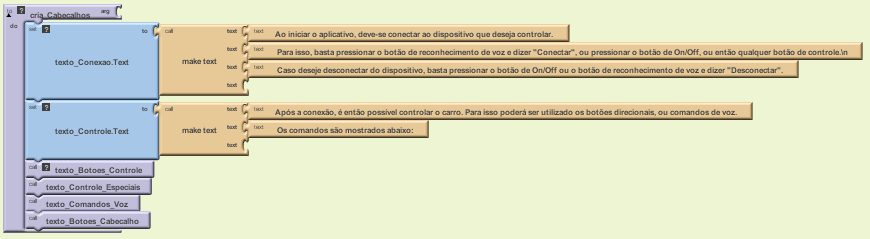
\includegraphics[scale=.7]{img/ajuda/cabecalho.png}
	
\end{figure}

\begin{verbatim}
Ao iniciar o aplicativo, deve-se conectar ao dispositivo que se deseja
 controlar.
Para isso, basta pressionar o botão de reconhecimento de voz e dizer 
"Conectar", ou pressionar o botão de On/Off, ou então qualquer botão 
de controle.
Caso deseje desconectar do dispositivo, basta pressionar o botão de 
On/Off ou o botão de reconhecimento de voz e dizer "Desconectar".

Após a conexão, é então possível controlar o caro. Para isso poderá 
ser utilizado os botões direcionais, ou comandos de voz.
Os comandos são mostrados abaixo:

\end{verbatim}

Após exibir um texto de introdução de ajuda ao usuário, a função criadora de textos (cabeçalhos) fará a ligação com os outros textos dividos no código por sessões:

\begin{itemize}
\item Botões de Controle Comuns;
\end{itemize}

\begin{figure}[H]
	\centering
	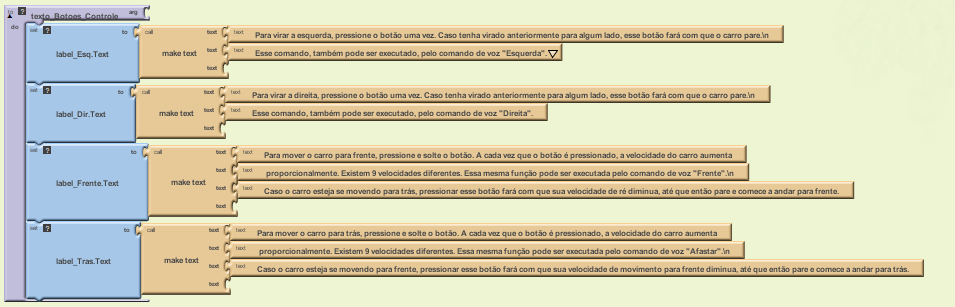
\includegraphics[scale=.7]{img/ajuda/controle.png}
	
\end{figure}
\begin{verbatim}
Para virar a esquerda, pressione o botão uma vez. Caso tenha virado 
anteriormente para algum lado, este botão fará com que o carro pare.
Este comando, também pode ser executado, pelo comando de voz "Esquerda".

Para virar a direita, pressione o botão uma vez. Caso tenha virado 
anteriormente para algum lado, este botão fará com que o carro pare.
Este comando, também pode ser executado, pelo comando de voz "Direita".

Para mover o carro para frente, pressione e solte o botão. A cada 
vez que o botão é pressionado, a velocidade do carro aumenta 
proporcionalmente. Exstem 9 velocidades diferentes. Essa mesma 
função pode ser executada pelo comando de voz "Frente".
Caso o carro esteja se movendo para trás, pressionar esse botão 
fará com que sua velocidade de ré diminua, até que então pare o 
carro e comece a andar para frente.

Para mover o carro para trás, pressione e solte o botão. A cada 
vez que o botão é pressionado, a velocidade do carro aumenta 
proporcionalmente. Exstem 9 velocidades diferentes. Essa mesma 
função pode ser executada pelo comando de voz "Afastar".
Caso o carro esteja se movendo para frente, pressionar esse botão 
fará com que sua velocidade de movimento para frente diminua, até 
que então pare o carro e comece a andar para trás.

\end{verbatim}

\begin{itemize}
\item Botões de Controle Especiais;
\end{itemize}
\begin{figure}[H]
	\centering
	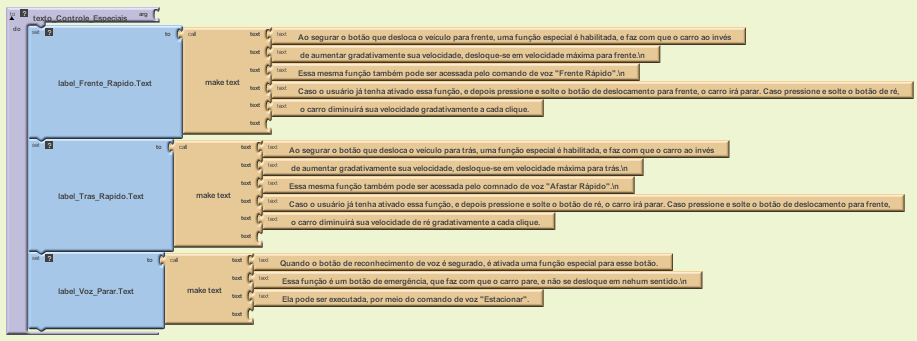
\includegraphics[scale=.7]{img/ajuda/especial.png}
	
\end{figure}
\begin{verbatim}
Ao segurar o botão que desloca o veículo para frente, uma função 
especial é habilitada, e faz com que o carro ao invés de 
aumentar gradativamente sua velocidade, desloque-se em 
velocidade máxima para frente.
Esta mesma função também pode ser acessada pelo comando de 
voz "Frente Rápido".
Caso o usuário já tenha ativado essa função, e depois pressione 
e solte o botão de deslocamento para frente, o caro irá parar. 
Caso pressione e solte o botão de ré, o carro diminuirá sua 
velocidade gradativamente a cada clique.

Ao segurar o botão que desloca o veículo para trás, uma função 
especial é habilitada, e faz com que o carro ao invés de aumentar 
gradativamente sua velocidade, desloque-se em velocidade máxima 
para trás.
Essa mesma função também pode ser acessada pelo comando de voz 
"Afastar Rápido".
Caso o usuário já tenha ativado essa função, e depois pressione 
e solte o botão de ré, o carro irá parar. Caso pressione e solte 
o botão de deslocamento para frente, o carro diminuirá sua 
velocidade de ré gradativamente a cada clicque.

Quando o boão de reconhecimento de voz é segurado, é ativada 
uma função especial para esse botão.
Essa função é um botão de emergência, que faz com que o carro 
pare, e não se desloque em nenhum sentido.
Ela pode ser executada, por meio do comando de voz "Estacionar".

\end{verbatim}

\begin{itemize}
\item Comandos de Voz;
\end{itemize}
\begin{figure}[H]
	\centering
	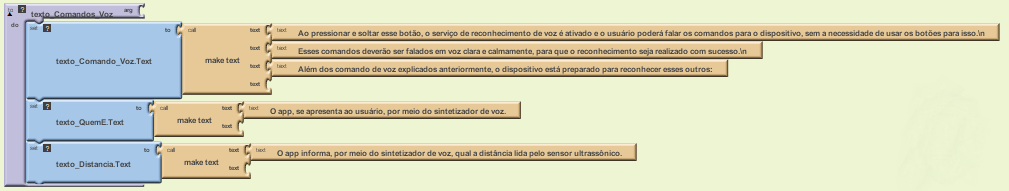
\includegraphics[scale=.7]{img/ajuda/voz.png}
	
\end{figure}
\begin{verbatim}
Ao pressionar e soltar esse botão, o serviço de reconhecimento 
de voz é ativado e o usuário poderá falar os comandos para o 
dispositivo, sem a necessidade de usar os botões para isso.
Esses comandos deverão ser falados em voz clara e calmamente, 
para que o reconhecimento seja realizado com sucesso.
Além dos comandos de voz explicados anteriormente, o 
dispositivo está preparado para reconhecer esses outro:

O app, se apresenta ao usuário, por meio do sintetizador de 
voz.

O app informa, por meio do sintetizador de voz, qual a distância 
lida pelo sensor ultrassônico.

\end{verbatim}
\begin{itemize}
\item Botões de Cabeçalho da tela.
\end{itemize}

\begin{figure}[H]
	\centering
	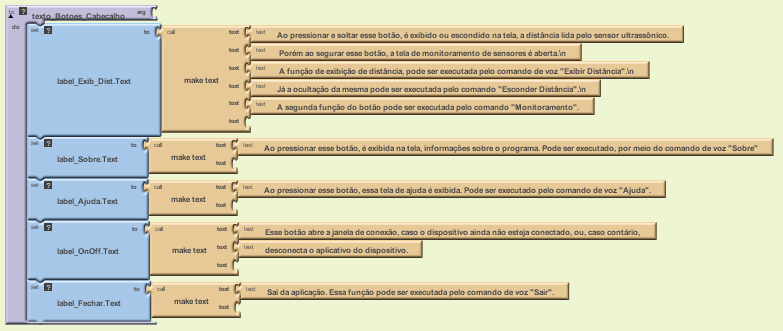
\includegraphics[scale=.8]{img/ajuda/bCabecalho.png}
	
\end{figure}
\begin{verbatim}
Ao pressionar e soltar esse botão, é exibido ou escondido na 
tela, a distância lida pelo sensor ultrassônico.
Porém ao segurar esse botão, a tela de monitoramento de sensores 
é aberta.

A função de exibição de distância, pode ser executada pelo 
comando de voz "Exibir Distância".

Já a ocultação da mesma pode ser executada pelo comando 
"Esconder Distância".
A segunda função do botão pode ser executada pelo comando
 "Monitoramento".

Ao pressionar esse botão, é exibida na tela, informações sobre 
o programa. Pode ser executado, por meio do comando de voz "Sobre".

Ao pressionar esse botão, essa tela de ajuda é exibida. Pode 
ser executado pelo comando de voz "Ajuda".

Esse botão abre a janela de conexão, caso o dispositivo ainda 
não esteja conectado, ou, contrário, desconecta o aplicativo do 
dispositivo.

Sai da aplicação. Essa função pode ser executada pelo comando de voz "Sair".

\end{verbatim}

\subsection{Fechando a janela Ajuda}
O procedimento realizado pelo \textit{software} de fechar a janela é bastante simples. Ele executa a vibração de cem milisegundos e em seguida a ação de fechar a janela.

\begin{figure}[H]
	\centering
	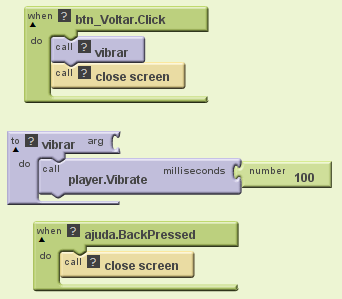
\includegraphics[scale=.8]{img/ajuda/saida.png}
	
\end{figure}



%%%%%%%%%%%%%%%%%%%%%%%%%%%%%%%%%%%%%%%%%%%%%%%%%%%%%%%%%%%%%%%%%%%%%%%%%%%%%%%%%%%%%%%%%%%%%%%%
%                                                                                              %
%                               Nova Seção do Documento                                        %
%                                                                                              %
%%%%%%%%%%%%%%%%%%%%%%%%%%%%%%%%%%%%%%%%%%%%%%%%%%%%%%%%%%%%%%%%%%%%%%%%%%%%%%%%%%%%%%%%%%%%%%%%

\newpage
\section{Ajuda da página de Monitoramento}
\subsection{Exibe textos do Monitoramento}
Semelhante ao procedimento de exibição da página Ajuda, neste procedimento serão chamados os textos que serão exibidos ao usuário, informando sobre como utilizar os componentes dessa tela.

\begin{figure}[H]
	\centering
	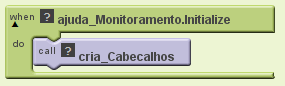
\includegraphics[scale=.8]{img/ajudaMonitoramento/inicio.png}
	
\end{figure}

\begin{figure}[H]
	\centering
	\includegraphics[scale=.7]{img/ajudaMonitoramento/cabecalho.png}

\end{figure}
\begin{verbatim}
Essa tela do app Carduino, é destinada à visualização das informações
dos sensores conectados ao carro.

As informações são atualizadas a cada segundo e apresentadas ao usuário.

\end{verbatim}


\begin{figure}[H]
	\centering
	\includegraphics[scale=.6]{img/ajudaMonitoramento/bCabecalho.png}

\end{figure}
\begin{verbatim}
Ao pressionar esse botão, é exibida na tela, informações sobre o
programa. Pode ser executado, por meio do comando de voz "Sobre".

Ao pressionar esse botão, essa tela de ajuda é exibida. Pode ser
executado pelo comando de voz "Ajuda.

Esse botão é usado para voltar a tela de controle, esse comando pode 
ser executado por meio dos comandos de voz:
"Voltar", "Fechar", "Sair", e "Controle".

\end{verbatim}


\begin{figure}[H]
	\centering
	\includegraphics[scale=.6]{img/ajudaMonitoramento/voz.png}

\end{figure}
\begin{verbatim}
Ao pressionar e soltar esse botão, o serviço de reconhecimento de voz
é ativado e o usuário poderá falar os comandos para o dispositivo,
sem a necessidade de usar botões para isso.

Esses comandos deverão ser falados em voz clara e calmamente, para que o
reconhecimento seja realizado com sucesso.

Além dos comandos de voz explicados anteriormente, o dispositivo está
preparado para reconhecer esses outros:

O app informa, por meio do sintetizador de voz, qual a distância lida
pelo sensor ultrassônico.

\end{verbatim}

\subsection{Fechando a janela Monitoramento}
O procedimento realizado pelo \textit{software} de fechar a janela que também é análogo ao da página Ajuda, se resume em uma vibração de cem milisegundos e em seguida executa a ação de fechar a janela.

\begin{figure}[H]
	\centering
	\includegraphics[scale=.8]{img/ajudaMonitoramento/saida.png}
	
\end{figure}




%%%%%%%%%%%%%%%%%%%%%%%%%%%%%%%%%%%%%%%%%%%%%%%%%%%%%%%%%%%%%%%%%%%%%%%%%%%%%%%%%%%%%%%%%%%%%%%%
%                                                                                              %
%                               Nova Seção do Documento                                        %
%                                                                                              %
%%%%%%%%%%%%%%%%%%%%%%%%%%%%%%%%%%%%%%%%%%%%%%%%%%%%%%%%%%%%%%%%%%%%%%%%%%%%%%%%%%%%%%%%%%%%%%%%

\newpage
\section{Página de Monitoramento}
\subsection{Variáveis}
Foi utilizado variáveis de inicialização para interligar os textos que serão apresentados na tela quando requisistados e valores de controle.


\begin{figure}[H]
	\centering
	\includegraphics[scale=.8]{img/monitoramento/variaveis.png}
	
\end{figure}

\subsection{Inicialização da Página}
Um procedimento de inicialização é executado na abertura da tela configurando todos os parâmetros necessário para o correto funcionamento da tela.

Primeiramente o sensor ultrassônico e a função \textit{sleep}\footnote{Função que faz uma pausa de alguns segundos por segurança na conexão.} são desativadas.

Logo em seguida são recuparados os valores passados por parâmetros através da tela principal. Além disso, como houve um troca de página, é necessário conectar novamente.
Após conectado, o procedimento é terminado mandando um comando para o carro robô para que ele retorne o valor da distância. Isso é feito para normalizar e inicializar os dados, pois ao serem lidos, não aparecerá um campo com o valor de distância ``vazia'' pois ele já terá lido um valor.

\begin{figure}[H]
	\centering
	\includegraphics[scale=.8]{img/monitoramento/inicializacao.png}
	
\end{figure}

\subsection{Principais Funções}
\subsubsection{Conectar}
Procedimento responsável por conectar ao carro robô. Como o \textit{software} já tem o endereço do dispositivo a ser conectado, ele reconecta automaticamente, ativando o recebimento dos dados do sensor ultrassônico.

\begin{figure}[H]
	\centering
	\includegraphics[scale=.8]{img/monitoramento/conectar.png}
	
\end{figure}

\subsubsection{Desconectar}
Função que torna a conexão com o sensor ultrassônico desligada sendo feito, logo em seguida, a desconexão com o carro robô.


\begin{figure}[H]
	\centering
	\includegraphics[scale=.8]{img/monitoramento/desconectar.png}
	
\end{figure}

\subsubsection{Botões}
Funções dos botões da página:
\begin{description}
\item [Voz:] Ativa o reconhecimento de voz do aplicativo;
\item [Voltar:] Volta a tela de controle do aplicativo;
\item [Sobre:] Abre a tela de informações do aplicativo;
\item [Ajuda:] Abre a tela de auxílio da tela de monitoramento;
\item [Voltar do Android:] Volta a tela de controle do aplicativo.
\end{description}


\begin{figure}[H]
	\centering
	\includegraphics[scale=.8]{img/monitoramento/btVoz.png}
	
\end{figure}
\begin{figure}[H]
	\centering
	\includegraphics[scale=.8]{img/monitoramento/btVoltar.png}
	
\end{figure}
\begin{figure}[H]
	\centering
	\includegraphics[scale=.8]{img/monitoramento/btSobre.png}
	
\end{figure}
\begin{figure}[H]
	\centering
	\includegraphics[scale=.8]{img/monitoramento/btAjuda.png}
	
\end{figure}
\begin{figure}[H]
	\centering
	\includegraphics[scale=.8]{img/monitoramento/monitoramentoBack.png}
	
\end{figure}

\subsubsection{Clock Conexão}
Este procedimento realiza a troca de tela de modo seguro análogo ao procedimento de mesmo nome da tela principal.


\begin{figure}[H]
	\centering
	\includegraphics[scale=.67]{img/monitoramento/clockConexao.png}
	
\end{figure}

\subsubsection{Clock Ultrassom}
Este procedimento é a junção da implementação dos procedimentos \verb%le_Distania% e \verb%clock_Ultrassom% da tela de controle (Sessão captada pelo Sensor).

\begin{figure}[H]
	\centering
	\includegraphics[scale=.7]{img/monitoramento/clockUltrassom.png}
	
\end{figure}

\subsubsection{Fechar a tela de monitoramento}
Responsável por fechar o aplicativo. Após a uma alerta de espera para o usuário (\verb%Aguarde um instante!%) este procedimento ativa a função \textit{sleep} para firmar um tempo para que possa se desconectar com total segurança.

\begin{figure}[H]
	\centering
	\includegraphics[scale=.8]{img/monitoramento/fechar.png}
	
\end{figure}


\subsubsection{Fala Distância}
Procedimento responsável por solicitar ao sintetizador de voz reproduza a distância, caso instalado.


\begin{figure}[H]
	\centering
	\includegraphics[scale=.8]{img/monitoramento/falaDistancia.png}
	
\end{figure}

\subsubsection{Chama Ajuda}
Procedimento responsável por abrir a janela de Ajuda da janela de Monitoramento para auxiliar os usuários ao utilizar os recursos dessa tela.

\begin{figure}[H]
	\centering
	\includegraphics[scale=.8]{img/monitoramento/chamaAjuda.png}
	
\end{figure}

\subsubsection{Vibrar}
Função responsável pela vibração do aparelho móvel. Isto só é possível se o dispositivo possuir essa função de vibração.

\begin{figure}[H]
	\centering
	\includegraphics[scale=.8]{img/monitoramento/vibrar.png}
	
\end{figure}

\subsection{Tocar Som}
Procedimento responsável por reproduzir os sons que serão executados pelo dispositivo móvel. 

É enviado por parâmentro o endereço do novo som. Por padrão, é definido que não será executada infinitas vezes, é executado o procedimento de vibração e em seguida a reprodução da música.

\begin{figure}[H]
	\centering
	\includegraphics[scale=.8]{img/monitoramento/abreSom.png}
	
\end{figure}

\subsubsection{Sobre}
Para abrir a janela do Sobre, é necessário inicar os comandos de sons, pois nela, há um música que toca ao fundo enquanto o usuário lê as informações sobre o aplicativo e seus responsáveis.

Por isso deve-se indicar qual música será executada, definir que será tocada sem parar (infinitas vezes). O procedimento também solicitará a função de vibração para alertar o usuário a mudança de página e assim, a tela Sobre é chamada.


\begin{figure}[H]
	\centering
	\includegraphics[scale=.8]{img/monitoramento/abreSobre.png}
	
\end{figure}

\subsubsection{Reconhecedor de Voz}
Procedimento responsável por verificar o som que o reconhecedor de voz gravou a partir do toque do usuário no botão deste evento.

Ele procurará entre todas as palavras da biblioteca do \textit{software} para executar-la se esta estiver correta.

\begin{description}
\item [Controle, Sair, Fechar, Voltar] Fecha a página de monitoramento e abre a página de Controle;
\item [Qual é a distância] Chama o procedimento responsável por reproduzir o valor da distância por meio do reconhecedor de voz;
\item [Ajuda] Chama o procedimento responsável por abrir a janela de Ajuda do usuário;
\item [Sobre] Chama o procedimento responsável por abrir a janela de Sobre;
\item [Quem é você] Chama o procedimento responsável pela apresentação do \textit{software}.
\end{description}

Deve-se lembrar que para que o reconhecedor de voz identifique e execute os comandos, deve-se pronunciar a palavra/frase numa velocidade lenta perante uma conversa cotidiana e em um volume médio. Não deve haver ruidos ao redor pois, tratando-se de um gravador comum, qualquer barulho terá consequência na verificação do som.

\begin{figure}[H]
	\centering
	\includegraphics[scale=.8]{img/monitoramento/ifs.png}
	
\end{figure}

\subsubsection{Telas Sobre}
Procedimentos que exibem a primeira e segunda tela de informações, e seus botões \verb%Sobre%, \verb%Mais%, \verb%Fechar% e \verb%Voltar%. O funcionamento deste procedimeto é análogo aos de mesmo nome da tela de monitoramento.

\begin{figure}[H]
	\centering
	\includegraphics[scale=.8]{img/monitoramento/sobre.png}
	
\end{figure}

\subsubsection{Botões tela Sobre}
Este procedimento é executado sempre que algum botão da tela Sobre é pressionado.

\begin{description}
\item[Fechar] Pausará a música;
\item[Mais] Chama a segunda tela;
\item[Voltar] Chama a primeira tela.
\end{description}


\begin{figure}[H]
	\centering
	\includegraphics[scale=.8]{img/monitoramento/voltarSobre.png}
	
\end{figure}

%%%%%%%%%%%%%%%%%%%%%%%%%%%%%%%%%%%%%%%%%%%%%%%%%%%%%%%%%%%%%%%%%%%%%%%%%%%%%%%%%%%%%%%%%%%%%%%%
%                                                                                              %
%                               Nova Seção do Documento                                        %
%                                                                                              %
%%%%%%%%%%%%%%%%%%%%%%%%%%%%%%%%%%%%%%%%%%%%%%%%%%%%%%%%%%%%%%%%%%%%%%%%%%%%%%%%%%%%%%%%%%%%%%%%

\newpage
%%%%%%%%%%% Example %%%%%%%%%%%%%%%%%%%%%%%%%%
\section{Bibliografia}
\begin{thebibliography}{100}

\bibitem{tuto} Tutorial: Criando aplicação para android para controlar o arduino através do bluetooth. Acessado 25/10/2013. Disponível em: http://labdegaragem.com/forum/topics/tutorial-criando-aplica-o-para-android-para-controlar-o-arduino?id=6223006\%3ATopic\%3A164130\&page=20


\bibitem{bt} BTArduinoLED1. Acessado 4/11/2013. Disponível em: http://ai.kittywolf.net/index.php/BTArduinoLED1


\bibitem{vibracall} Como funciona o Vibracall. Acessado 7/11/2013. Disponível em: http://super.abril.com.br/tecnologia/como-funciona-vibracall-619305.shtml.

\end{thebibliography}

\end{document}